\chapter{Enemies and their Discontents} 
\label{sec:level}

\lstset{style=6502Style}

\begin{q}{Jeff Minter's Development Diary in Zzap Magazine\cite{planner}}
ACONT 

This is the bit that I knew would take me ages to write and get glitch
free, and the bit that is absolutely necessary to the functioning of the game.
The module ACONT is essentially an interpreter for my own 'wave language',
allowing me to describe, exactly, an attack wave in about 50 bytes of data. The
waves for the first part of IRIDIS are in good rollicking shoot-'em-up style,
and there have to be plenty of them. There are five planets and each planet is
to have twenty levels associated with it. It's impractical to write separate
bits of code for each wave; even with 64K you can run outta memory pretty fast
that way, and it's not really necessary coz a lot of stuff would be duplicated.
Hence ACONT.

\end{q}

The bits and bytes that define the behaviour and appearance of
wave after wave of Iridis Alpha's enemy formations - twenty across each of the
five planets giving one hundred in all - takes up relatively little space given
the sheer variety of adversaries the player faces.


\begin{figure}[H]
  {
    \setlength{\tabcolsep}{3.0pt}
    \setlength\cmidrulewidth{\heavyrulewidth} % Make cmidrule = 
	\centering
	\begin{subfigure}{0.3\textwidth}
    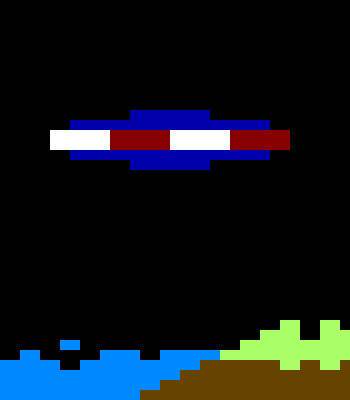
\includegraphics[width=2cm]{src/sprites/gallery/sprite_160.png}%
	\end{subfigure}
	\begin{subfigure}{0.3\textwidth}
    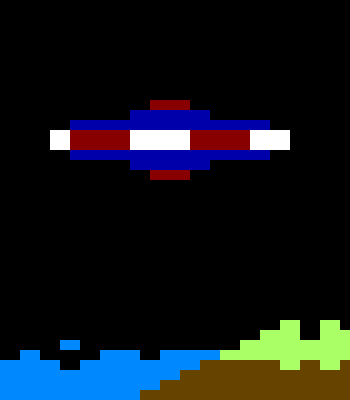
\includegraphics[width=2cm]{src/sprites/gallery/sprite_161.png}%
	\end{subfigure}
	\begin{subfigure}{0.3\textwidth}
    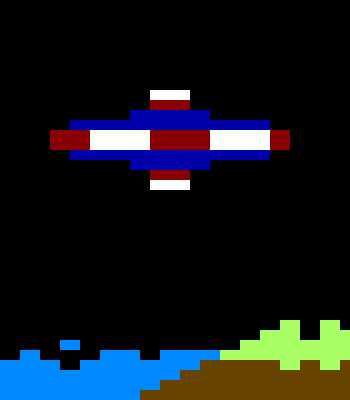
\includegraphics[width=2cm]{src/sprites/gallery/sprite_162.png}%
	\end{subfigure}
  }

  {
  \setlength{\tabcolsep}{3.0pt}
  \setlength\cmidrulewidth{\heavyrulewidth} % Make cmidrule = 
  \begin{adjustbox}{width=13cm}

\begin{tabular}{lll}
\toprule
 Byte    & Value                     & Description                                                        \\
\midrule
  Byte 0  & \icode{\$06}                       & Index into array for sprite color                                  \\
 Byte 1  & FLYING\_SAUCER1            & First sprite value for the attack ship on the upper planet               \\
 Byte 2  & FLYING\_SAUCER3            & Last sprite value for the attack ship on the upper planet               \\
 Byte 3  & \$03                       & The animation frame rate for the attack ship.                      \\
 Byte 4  & FLYING\_SAUCER1            & First sprite value for the attack ship on the lower planet               \\
 Byte 5  & FLYING\_SAUCER3            & Last sprite value for the attack ship on the lower planet               \\
 Byte 6  & \$00                       & Rate at which to switch to alternate enemy mode.                       \\
 Byte 7  & nullPtr                   & Lo Ptr for alternate enemy mode                             \\
 Byte 8  & nullPtr                   & Hi Ptr for alternate enemy mode                             \\
 Byte 9  & nullPtr                   & \textbf{Unused} Lo Ptr to an arbitrary run of Bytes 18-21.\\
 Byte 10 & nullPtr                   & \textbf{Unused} Hi Ptr to an arbitrary run of Bytes 18-21.\\
 Byte 11 & \$00                       & \textbf{Unused} Rate limite for use of Bytes 9 and 10. \\
 Byte 12 & nullPtr                   & \textbf{Unused} \\
 Byte 13 & nullPtr                   & \textbf{Unused} \\
 Byte 14 & \$00                       & Controls the rate at which new enemies are added.\\
 Byte 15 & \$40                       & Update rate for attack wave                                        \\
 Byte 16 & planet1Level1Data2ndStage & Lo Ptr to the wave data we switch to when first hit.               \\
 Byte 17 & planet1Level1Data2ndStage & Hi Ptr to the wave data we switch to when first hit.               \\
 Byte 18 & \$06                       & X Pos movement for attack ship.                                    \\
 Byte 19 & \$01                       & Y Pos movement pattern for attack ship.                            \\
 Byte 20 & \$01                       & X Pos Frame Rate for Attack ship.                                  \\
 Byte 21 & \$01                       & Y Pos Frame Rate for Attack ship.                                  \\
 Byte 22 & \$00                       & Stickiness factor, does the enemy stick to the player              \\
 Byte 23 & \$00                       & Does the enemy gravitate quickly toward the player when its hit?   \\
 Byte 24 & nullPtr                   & Lo Ptr for second wave of attack ships.                               \\
 Byte 25 & nullPtr                   & Hi Ptr for second wave of attack ships.                               \\
 Byte 26 & nullPtr                   & Lo Ptr for third wave of attack ships.                               \\
 Byte 27 & nullPtr                   & Hi Ptr for third wave of attack ships.                               \\
 Byte 28 & spinningRings             & Lo Ptr for Explosion animation.                                    \\
 Byte 29 & spinningRings             & Hi Ptr for Explosion animation.                                    \\
 Byte 30 & defaultExplosion          & Lo Ptr for another set of wave data for this level.                \\
 Byte 31 & defaultExplosion          & Hi Ptr for another set of wave data for this level.                \\
 Byte 32 & \$00                       & Lo Ptr for fourth wave of attack ships.                                                            \\
 Byte 33 & \$00                       & Hi Ptr for fourth wave of attack ships.                           \\
 Byte 34 & \$02                       & Points for hitting the enemy. \\
 Byte 35 & \$02                       & Energy increase multiplier for hitting an enemy.\\
 Byte 36 & \$00                       & Is the ship a spinning ring, i.e. does it allow the gilby to warp? \\
 Byte 37 & \$04                       & Number of waves in data.                                           \\
 Byte 38 & \$18                       & Number of ships in wave.                                           \\
 Byte 39 & \$00                       & \textbf{Unused} byte.                                                      \\
\bottomrule
\end{tabular}

  \end{adjustbox}

  }\caption*{Sheep Planet - Level 1 - Enemy Data for the First Wave.}
\end{figure}
\clearpage

\section{Something Simple - Byte 0: The Enemy's Color}
To get an understanding of how the level data is used we can start with the very first byte of the data
used for the first wave in the very first level. This is the wave of flying saucers you will already be
familiar with if you have played the game (:)):
\begin{figure}[H]
  {
    \setlength{\tabcolsep}{3.0pt}
    \setlength\cmidrulewidth{\heavyrulewidth} % Make cmidrule = 
	\centering
	\def\MULTICOLORONE{white}
	\def\MULTICOLORTWO{red}
	\def\SPRITECOLOR{blue}
	\begin{subfigure}{0.3\textwidth}
		\input{sprites/FLYING_SAUCER1}
	\end{subfigure}
	\begin{subfigure}{0.3\textwidth}
		\input{sprites/FLYING_SAUCER2}
	\end{subfigure}
	\begin{subfigure}{0.3\textwidth}
		\input{sprites/FLYING_SAUCER3}
	\end{subfigure}
  }\caption[position=top]{The sprites used to animate the 'UFO' in the first level.}
\end{figure}

The main colour for this sprite is blue. This may not be obvious from looking at the sprites themselves, but
the way the sprite color schemes work is that you can select two colors that are available for all sprites and
one color that is unique to the sprite itself. In this case, the unique color selected for the flying saucers is
determined by Byte 1 in the Level Data. You can see in the table in the page opposite
that this is defined with a value of \icode{\$06}. This is how it looks in the code itself:

\begin{lstlisting}
planet1Level1Data
    ; Byte 0 (Index $00): An index into colorsForAttackShips that applies a
    ; color value for the ship sprite.
    .BYTE $06
\end{lstlisting}

This value is an index into the array \icode{colorsForAttackShips}. Starting at zero we count up to 6
and arrive at the 7th item in the list below, giving us the result \icode{BLUE}:
\begin{lstlisting}
colorsForAttackShips
    .BYTE BLACK,WHITE,RED,CYAN,PURPLE,GREEN,BLUE,YELLOW
    .BYTE ORANGE,BROWN,LTRED,GRAY1,GRAY2,LTGREEN,LTBLUE,GRAY3
\end{lstlisting}

In the routine that draws the attack wave we find the following code segment writing this value
to the register \icode{\$D027} that determines the color of the sprite:

\begin{lstlisting}
;-------------------------------------------------------
; DrawUpperPlanetAttackShips Routine
;-------------------------------------------------------
DrawUpperPlanetAttackShips
    LDX #$0C
    LDY #$06
UpperPlanetShipsLoop   
    ...
    LDX upperPlanetAttackShipsColorArray,Y
    LDA colorsForAttackShips,X
    STA $D027,Y  ;Sprite Y Color
    ...
    DEX
    DEX
    DEY
    BNE UpperPlanetShipsLoop
    RTS
\end{lstlisting}

Notice that the \icode{\$06} was originally stored in a position in the array \icode{upperPlanetAttackShipsColorArray}.
This happened in an earlier routine that loads the majority of the data for a level:


\begin{lstlisting}
GetWaveDataForNewShip
    ; X is the index of the ship in activeShipsWaveDataLoPtrArray
    LDY #$00
    LDA (currentShipWaveDataLoPtr),Y
    STA upperPlanetAttackShipsColorArray + $01,X
\end{lstlisting}

\section{Bytes 1-4: Sprite Animation}
\begin{q}{Jeff Minter's Development Diary in Zzap Magazine\cite{planner}}
You pass the interpreter data, that describes exactly stuff like: what each
alien looks like, how many frames of animation it uses, speed of that
animation, colour, velocities in X— and Y— directions, accelerations in X and
Y, whether the alien should 'home in' on a target, and if so, what to home in
on; whether an alien is subject to gravity, and if so, how strong is the
gravity; what the alien should do if it hits top of screen, the ground, one of
your bullets, or you; whether the alien can fire bullets, and if so, how
frequently, and what types; how many points you get if you shoot it, and how
much damage it does if it hits you; and a whole bunch more stuff like that. As
you can imagine it was a fairly heavy routine to write and get debugged, but
that's done now; took me about three weeks in all I'd say.
\end{q}

\begin{figure}[H]
  {
    \setlength{\tabcolsep}{3.0pt}
    \setlength\cmidrulewidth{\heavyrulewidth} % Make cmidrule = 
	\centering
	\def\MULTICOLORONE{red}
	\def\MULTICOLORTWO{white}
	\def\SPRITECOLOR{orange}
	\begin{subfigure}{0.3\textwidth}
		\input{sprites/CUMMING_COCK1}
	\end{subfigure}
	\begin{subfigure}{0.3\textwidth}
		\input{sprites/CUMMING_COCK2}
	\end{subfigure}
	\begin{subfigure}{0.3\textwidth}
		\input{sprites/CUMMING_COCK3}
	\end{subfigure}
  }\caption[position=top]{Confirmation that the game developer was a young male. The sprites used to animate attack wave 17 in the Mushroom Planet.}
\end{figure}

Looking again at the table in the previous page we can see the first 7 bytes are concerned with the appearance and basic behaviour of the
enemy. Bytes 1 and 2 define the sprite used for display on the upper planet, Bytes 4 and 5
for the lower planet. The reason there's two in each case is because they are describing the
start and end point of the sprite's animation. 

We can see this in action in \icode{AnimateAttackShipSprites}. When this routine runs Byte 3 has been loaded
to \icode{upperPlanetAttackShipInitialFrameRate} for the upper planet and \icode{lowerPlanetAttackShipInitialFrameRate}
for the lower planet. This routine is cycling through the sprites given by Byte 1 as the lower limit and Byte 2 as 
the upper limit. This is what the animation consists of: an animation effect achieved by changing the sprite from
one to another to create a classic animation effect.

\begin{lstlisting}[caption=Routine for Animating Enemy Sprites. ]
AnimateAttackShipSprites
    LDA pauseModeSelected
    BEQ AnimateUpperPlanetAttackShips
    RTS

AnimateUpperPlanetAttackShips   
    DEC upperPlanetAttackShipAnimationFrameRate - $01,X
    BNE AnimateLowerPlanetAttackShips

    LDA upperPlanetAttackShipInitialFrameRate - $01,X
    STA upperPlanetAttackShipAnimationFrameRate - $01,X
    INC upperPlanetAttackShip2SpriteValue,X
    LDA upperPlanetAttackShip2SpriteValue,X

    ; Reached the end of the animation?
    CMP upperPlanetAttackShipSpriteAnimationEnd - $01,X
    BNE AnimateLowerPlanetAttackShips

    ; Reset the animation sprite back to the start.
    LDA upperPlanetAttackShipSpritesLoadedFromBackingData - $01,X
    STA upperPlanetAttackShip2SpriteValue,X

AnimateLowerPlanetAttackShips   
    DEC lowerPlanetAttackShipAnimationFrameRate - $01,X
    BNE DontAnimateLowerPlanetAttackShip

    LDA lowerPlanetAttackShipInitialFrameRate - $01,X
    STA lowerPlanetAttackShipAnimationFrameRate - $01,X
    INC lowerPlanetAttackShip2SpriteValue,X
    LDA lowerPlanetAttackShip2SpriteValue,X

    ; Reached the end of the animation?
    CMP lowerPlanetAttackShipSpriteAnimationEnd - $01,X
    BNE DontAnimateLowerPlanetAttackShip

    ; Reset the animation sprite back to the start.
    LDA lowerPlanetAttackShipSpritesLoadedFromBackingData - $01,X
    STA lowerPlanetAttackShip2SpriteValue,X
DontAnimateLowerPlanetAttackShip   
    RTS
\end{lstlisting}
 
Byte 1 (loaded to \icode{upperPlanetAttackShipAnimationFrameRate} comes into play here. It's decremented and as long as it's
not zero yet the animation is skipped, execution jumps forward to \icode{AnimateLowerPlanetAttackShips}:

\begin{lstlisting}
AnimateLowerPlanetAttackShips   
    DEC lowerPlanetAttackShipAnimationFrameRate - $01,X
    BNE DontAnimateLowerPlanetAttackShip

    LDA lowerPlanetAttackShipInitialFrameRate - $01,X
    STA lowerPlanetAttackShipAnimationFrameRate - $01,X
    INC lowerPlanetAttackShip2SpriteValue,X
    LDA lowerPlanetAttackShip2SpriteValue,X

    ; Reached the end of the animation?
    CMP lowerPlanetAttackShipSpriteAnimationEnd - $01,X
    BNE DontAnimateLowerPlanetAttackShip

    ; Reset the animation sprite back to the start.
    LDA lowerPlanetAttackShipSpritesLoadedFromBackingData - $01,X
    STA lowerPlanetAttackShip2SpriteValue,X
\end{lstlisting}

If it is zero, it instead gets reset to the initial value from Byte 1 (stored in
 \icode{upperPlanet\-AttackShipInitialFrameRate})
and the current sprite for the enemy ship is incremented to point to the next 'frame' of the ship's animation:

\begin{lstlisting}
AnimateUpperPlanetAttackShips   
    DEC upperPlanetAttackShipAnimationFrameRate - $01,X
    BNE AnimateLowerPlanetAttackShips

    LDA upperPlanetAttackShipInitialFrameRate - $01,X
    STA upperPlanetAttackShipAnimationFrameRate - $01,X
    INC upperPlanetAttackShip2SpriteValue,X
    LDA upperPlanetAttackShip2SpriteValue,X

    ; Reached the end of the animation?
    CMP upperPlanetAttackShipSpriteAnimationEnd - $01,X
    BNE AnimateLowerPlanetAttackShips

    ; Reset the animation sprite back to the start.
    LDA upperPlanetAttackShipSpritesLoadedFromBackingData - $01,X
    STA upperPlanetAttackShip2SpriteValue,X
\end{lstlisting}

Next we check if we've reached the end of the animation by checking the value
of Byte 2 (loaded to \icode{upperPlanetAttackShipSpriteAnimationEnd}).  If so,
we reset \icode{upperPlanetAttackShip2SpriteValue} to the value initially
loaded from Byte 1 - and that is what will be used to display the ship the next
time we pass through to animate the ship:

\begin{lstlisting}
DrawUpperPlanetAttackShips
    LDX #$0C
    LDY #$06
UpperPlanetShipsLoop   
    LDA upperPlanetAttackShipsXPosArray,Y
    STA $D000,X  ;Sprite 0 X Pos

    LDA attackShipsXPosArray - $01,Y
    AND $D010    ;Sprites 0-7 MSB of X coordinate
    STA currentMSBXPosOffset

    LDA upperPlanetAttackShipsMSBXPosArray,Y
    AND attackShipsMSBXPosOffsetArray,Y
    ORA currentMSBXPosOffset
    STA $D010    ;Sprites 0-7 MSB of X coordinate

    LDA upperPlanetAttackShipsYPosArray,Y
    STA $D001,X  ;Sprite 0 Y Pos
    STX tempVarStorage

    LDX upperPlanetAttackShipsColorArray,Y
    LDA colorsForAttackShips,X
    STA $D027,Y  ;Sprite 0 Color

    LDA upperPlanetAttackShipsSpriteValueArray,Y
    STA Sprite0Ptr,Y
    LDX tempVarStorage

    DEX
    DEX
    DEY
    BNE UpperPlanetShipsLoop
    RTS
\end{lstlisting}

\section{Bytes 18-21: Enemy Movement}

Enemy movement is controlled by two parameters in each direction: the number of pixels to move in one go and the number of
cycles to wait between each movement. So for movement in the horizontal (or X direction) \icode{Byte 18} controls the number
of pixels to move at once, while \icode{Byte 20} controls the number of cycles to wait between each movement. The same
applies to \icode{Byte 19} and \icode{Byte 21} for the vertical (or Y direction).

If we look at Byte 18 and Byte 20 for Level 1 we can see that the the fast lateral movement of the 'UFO's is implemented by a relatively
high value of \$06 for the number of pixels it moves at each step while the interval between steps is relatively low (\$01).
Meanwhile the more gradual up and down movement is implemented by a value of \$01 in Byte 19 and Byte 21.

For the second level ('bouncing rings') the horizontal movement is more constrained (Byte 18 is \$00) while the vertical movement
is more extreme (Byte 19 is \$24) - achieving the bouncing effect.



\begin{figure}[H]
  {
    \setlength{\tabcolsep}{3.0pt}
    \setlength\cmidrulewidth{\heavyrulewidth} % Make cmidrule = 
    \begin{adjustbox}{width=8cm,center}

      \begin{tabular}{rlllll}
        \toprule
        Level & Byte 6    & Byte 18   & Byte 19   & Byte 20   & Byte 21   \\
        \midrule
        1 & \$00       & \$06       & \$01       & \$01       & \$01       \\
        2 & \$00       & \$00       & \$24       & \$02       & \$01       \\
        3 & \$00       & \$FA       & \$01       & \$01       & \$02       \\
        \addlinespace
        \bottomrule
        \multicolumn{6}{@{}l@{}}{Byte 6 : Whether a specific attack behaviour is used.}\\
        \multicolumn{6}{@{}l@{}}{Byte 18: X Pos movement for attack ship.}\\
        \multicolumn{6}{@{}l@{}}{Byte 19: Y Pos movement pattern for attack ship.}\\
        \multicolumn{6}{@{}l@{}}{Byte 20: X Pos Frame Rate for Attack ship.}\\
        \multicolumn{6}{@{}l@{}}{Byte 21: Y Pos Frame Rate for Attack ship.}\\
      \end{tabular}

    \end{adjustbox}

    }\caption*{Movement data for the first three levels.}
\end{figure}

The horizontal movement for Level Three, home to the infamous 'Licker Ships' is \$FA, which would make you think the enemies must be moving horizontally
extremely quickly. In fact, when the high bit is set a special behaviour is invoked:

\begin{lstlisting}[caption=From \icode{UpdateAttackShipsXAndYPositions}.  ]
        LDA xPosMovementForUpperPlanetAttackShip - $01,X
        BMI UpperBitSetOnXPosMovement
\end{lstlisting}

This is the special behaviour that makes the Licker Ships on this level such an enormous pain in the arse to play against.

\begin{figure}[H]
    \centering
    \foreach \l in {0,...,1}
    {
      \includegraphics[width=6cm]{level_data/images/movement_1_3_\l.png}%
    }%
\caption*{Enemy movement for Sheep planet, level 3 - the infamous licker ships.}
\end{figure}

When the upper bit is set (e.g. \$FC,\$80) on the value loaded to the accumulator by \icode{LDA} then \icode{BMI} will 
return true and jump to \icode{UpperBitSetOnXPosMovement}.

\begin{lstlisting}
UpperBitSetOnXPosMovement   
        ; This creates a decelerating effect on the attack ship's movement.
        ; Used by the licker ship wave in planet 1 for example.
        EOR #$FF
        STA attackShipOffsetRate
        INC attackShipOffsetRate
        LDA upperPlanetAttackShip2XPos,X
        SEC
        SBC attackShipOffsetRate
        STA upperPlanetAttackShip2XPos,X
        BCS DecrementXPosFrameRateLowerPlanet

        LDA upperPlanetAttackShip2MSBXPosValue,X
        EOR attackShip2MSBXPosOffsetArray,X
        STA upperPlanetAttackShip2MSBXPosValue,X
\end{lstlisting}

This first line \icode{EOR \#\$FF} performs an exclusive-or between Byte 19 in the \icode{Accumulator} (\$FA) and the value \$FF. An exclusive-or,
remember, is a bit by bit comparison of two bytes which will set a bit in the result if an only if the bit in one of the
values is set but the other is not:

\begin{figure}[H]
  {
    \setlength{\tabcolsep}{3.0pt}
    \setlength\cmidrulewidth{\heavyrulewidth} % Make cmidrule = 
    \begin{adjustbox}{width=7cm,center}

      \begin{tabular}{rllllllll}
        \toprule
        Byte & Bit 7 & Bit 6 & Bit 5 & Bit 4 & Bit 3 & Bit 2 & Bit 1 & Bit 0        \\
        \midrule
        \$FF & 1 & 1 & 1 & 1 & 1 & 1 & 1 & 1 \\
        \$FA & 1 & 1 & 1 & 1 & 1 & 0 & 1 & 0 \\
        \midrule
        Result & 0 & 0 & 0 & 0 & 0 & 1 & 0 & 1 \\
        \addlinespace
        \bottomrule
      \end{tabular}

    \end{adjustbox}

    }\caption*{X-OR'ing \$FF and \$FA gives \$05.}
\end{figure}

This result is stored in \icode{attackShipOffsetRate}:
\begin{lstlisting}
UpperBitSetOnXPosMovement   
  ; This creates a decelerating effect on the attack ship's movement.
  ; Used by the licker ship wave in planet 1 for example.
  EOR #$FF
  STA attackShipOffsetRate
\end{lstlisting}

Incremented:
\begin{lstlisting}
        INC attackShipOffsetRate
\end{lstlisting}

And then subtracted from the enemy's X position:
\begin{lstlisting}
  SEC
  SBC attackShipOffsetRate
  STA upperPlanetAttackShip2XPos,X
\end{lstlisting}

The net result is a deceleration effect. This is observed in the way the licker ship
wave will accelerate out to the center before dialling back again.


\subsection{What is going on with Byte 6?}

Byte 6 comes into play when setting the initial Y position of a new enemy. This initial vertical
position is random, but subject to some adjustment:

\begin{lstlisting}[caption=The sub-routine \icode{SetInitialRandomPositionUpperPlanet} in \icode{GetWaveDateForNewShip}.  ]
SetInitialRandomPositionUpperPlanet   
  JSR PutProceduralByteInAccumulatorRegister
  AND #$3F
  CLC
  ADC #$40
  STA upperPlanetAttackShipsYPosArray + $01,Y

  STY previousAttackShipIndexTmp
  ; Byte 6 ($06): Usually an update rate for the attack ships.
  LDY #$06
  LDA (currentShipWaveDataLoPtr),Y
  BNE ReturnFromLoadingWaveDataEarly

  ; Byte 8 ($08): Default initiation Y position for the enemy. 
  LDY #$08
  LDA (currentShipWaveDataLoPtr),Y
  BEQ ReturnFromLoadingWaveDataEarly

  LDA #$6C
  LDY previousAttackShipIndexTmp
  STA upperPlanetAttackShipsYPosArray + $01,Y

ReturnFromLoadingWaveDataEarly   
  RTS
\end{lstlisting}

The first order of business is to call \icode{PutProceduralByteInAccumulatorRegister} which gets a random value and stores it in the accumulator.

\begin{lstlisting}
PutProceduralByteInAccumulatorRegister
randomIntToIncrement   =*+$01
    LDA randomPlanetData
    INC randomIntToIncrement
    RTS
\end{lstlisting}

Since \icode{A} can now contain anything from 0 to 255 (\$00 to \$FF) this needs to be adjusted to a meaningful Y-position
value for the upper planet. So if we imagine \icode{PutProceduralByteInAccumulatorRegister} returned \$85, we now do the
following operations on it:

\begin{lstlisting}
        AND #$3F
        CLC
        ADC #$40
        STA upperPlanetAttackShipsYPosArray + $01,Y
\end{lstlisting}

First we do an \icode{AND \#\$3F} with the value of \$85 in \icode{A}:
\begin{figure}[H]
  {
    \setlength{\tabcolsep}{3.0pt}
    \setlength\cmidrulewidth{\heavyrulewidth} % Make cmidrule = 
    \begin{adjustbox}{width=10cm,center}

      \begin{tabular}{rllllllll}
        \toprule
        Byte & Bit 7 & Bit 6 & Bit 5 & Bit 4 & Bit 3 & Bit 2 & Bit 1 & Bit 0        \\
        \midrule
        \$85 & 1 & 0 & 0 & 0 & 0 & 1 & 0 & 1 \\
        \$3F & 0 & 0 & 1 & 1 & 1 & 1 & 1 & 1 \\
        \midrule
        Result & 0 & 0 & 0 & 0 & 0 & 1 & 0 & 1 \\
        \addlinespace
        \bottomrule
      \end{tabular}

    \end{adjustbox}

    }\caption*{AND'ing \$3F and \$85 gives \$05.}
\end{figure}

Our result is \$05. The effect of the AND'ing here is to ensure that the random number we get back is between 0 and 63 rather
than 0 and 255. Next we add \$40 (decimal 64) to this result:

\begin{lstlisting}
        CLC
        ADC #$40
\end{lstlisting}

This gives \$45 and this is what we store as the initial Y position for the enemy.

You'll notice that the steps for \icode{SetInitialRandomPositionLowerPlanet} are identical but with only the constant of the
add value of \$98 instead of \$40. This is simply an additional offset to ensure that the Y position is lower on the screen
for the initial position of the enemy on the lower planet.

We still haven't got into what Byte 7 is doing though. With an initial Y position determined, it looks like the intention was
for Byte 6 to specify some adjustment to this value. But this looks like another bit of non-functioning game logic. If
Byte 6 contains a value, the function will return early without any further adjustments. If it's zero it will then try
Byte 8. If that's zero, it will return early. So the logic needs Byte 6 to be zero and Byte 8 to contain something for 
anything to happen. That's never the case, so the the adjustment never happens:

\begin{lstlisting}[caption= An adjustment that never happens. Byte 6 and Byte 8 are never set in this way.]
        STY previousAttackShipIndexTmp
        ; Byte 6 ($06): Usually an update rate for the attack ships.
        LDY #$06
        LDA (currentShipWaveDataLoPtr),Y
        BNE ReturnFromLoadingWaveDataEarly

        ; Byte 8 ($08): Default initiation Y position for the enemy. 
        LDY #$08
        LDA (currentShipWaveDataLoPtr),Y
        BEQ ReturnFromLoadingWaveDataEarly
\end{lstlisting}

This is definitely some forgotten code. Byte 6 is elsewhere used in combination with Byte 7 and Byte 8 to define an alternate
enemy mode for some levels where the ship will supplement any dead ships with alternate enemy types and attack patterns periodically.


\section{Bytes 6-8: Alternate Enemy Waves}
This happens in \icode{MaybeSwitchToAlternateEnemyPattern} in \icode{UpdateAttackShipDataForNewShip}. 

\begin{lstlisting}[caption=Byte 6 is used to periodically switch to an enemy mode defined by Bytes 7-8 ]
MaybeSwitchToAlternateEnemyPattern   
        ; Byte 6 ($06): Usually an update rate for the attack ships.
        LDY #$06
        LDA (currentShipWaveDataLoPtr),Y
        BEQ EarlyReturnFromAttackShipBehaviour

        DEC rateForSwitchingToAlternateEnemy,X
        BNE EarlyReturnFromAttackShipBehaviour

        LDA (currentShipWaveDataLoPtr),Y
        STA rateForSwitchingToAlternateEnemy,X

        ; Push the current ship's position data onto the stack.
        TXA
        PHA
        LDY indexIntoUpperPlanetAttackShipXPosAndYPosArray,X
        LDA upperPlanetAttackShipsXPosArray + $01,Y
        PHA
        LDA upperPlanetAttackShipsMSBXPosArray + $01,Y
        PHA
        LDA upperPlanetAttackShipsYPosArray + $01,Y
        PHA

        ; Are we on the top or bottom planet?
        TXA
        AND #$08
        BNE LowerPlanetAttackShipBehaviour

\end{lstlisting}

Byte 6 is used to drive the rate at which this routine switches over to the enemy data/mode defined by Byte 7 and Byte 8.

\begin{lstlisting}[caption=\icode{rateForSwitchingToAlternateEnemy} (Byte 6) is decremented and reloaded each time it reaches zero. ]
        DEC rateForSwitchingToAlternateEnemy,X
        BNE EarlyReturnFromAttackShipBehaviour

        LDA (currentShipWaveDataLoPtr),Y
        STA rateForSwitchingToAlternateEnemy,X
\end{lstlisting}

What this routine is going to do is replace the first dead ship it finds in the current wave with the wave data pointed to by  Byte 7-8
and create a new enemy with the current ship's position with it.

First, we store the current ship's position. The way to do this is get the index (\icode{Y}) for the current ship \icode{X} and store
each of the X and Y Position information into the accumulator first \icode{A} and then push it onto the 'stack' (\icode{PHA} which means
'push \icode{A} onto the stack').

\begin{lstlisting}
        ; Push the current ship's position data onto the stack.
        TXA
        PHA
        LDY indexIntoUpperPlanetAttackShipXPosAndYPosArray,X
        LDA upperPlanetAttackShipsXPosArray + $01,Y
        PHA
        LDA upperPlanetAttackShipsMSBXPosArray + $01,Y
        PHA
        LDA upperPlanetAttackShipsYPosArray + $01,Y
        PHA
\end{lstlisting}

When this has run the stack of accumulator values now looks like this:

\begin{figure}[H]
  {
    \setlength{\tabcolsep}{3.0pt}
    \setlength\cmidrulewidth{\heavyrulewidth} % Make cmidrule = 
    \begin{adjustbox}{width=10cm,center}
      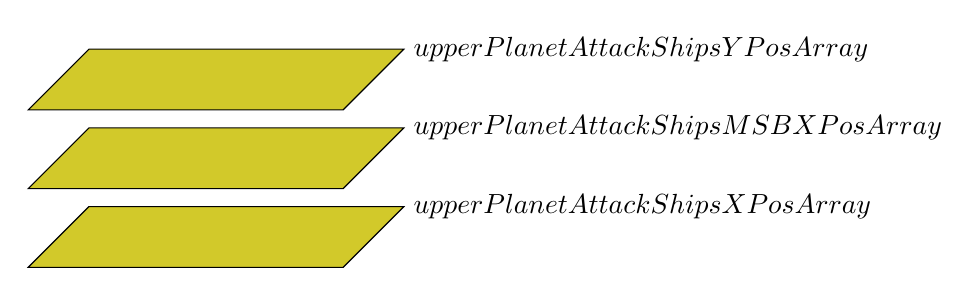
\begin{tikzpicture}
      \draw[fill=yellow!80!black] (0,1,0) -- (4,1,0)--(4,1,2)--(0,1,2)--cycle;
      \node[right] at (4,1,0) {$\icode{upperPlanetAttackShipsXPosArray}$};
      \draw[fill=yellow!80!black] (0,2,0) -- (4,2,0)--(4,2,2)--(0,2,2)--cycle;
      \node[right] at (4,2,0) {$\icode{upperPlanetAttackShipsMSBXPosArray}$};
      \draw[fill=yellow!80!black] (0,3,0) -- (4,3,0)--(4,3,2)--(0,3,2)--cycle;
      \node[right] at (4,3,0) {$\icode{upperPlanetAttackShipsYPosArray}$};
      \end{tikzpicture}
    \end{adjustbox}

  }\caption*{The stack after the code above has run with \icode{upperPlanetAttackShipsXPosArray} at the top.}
\end{figure}

With our position data safely stashed away on the stack we now decide which planet we're on:

\begin{lstlisting}[caption= ]
        ; Are we on the top or bottom planet?
        TXA
        AND #$08
        BNE LowerPlanetAttackShipBehaviour
\end{lstlisting}

If we're on the upper planet we use \icode{SetXToIndexOfShipThatNeedsReplacing} look in the \icode{activeShipsWaveDataHiPtrArray} for any ships that
need replacing between positions \icode{\$02} and \icode{\$06}. If we don't find one, we return early:

\begin{lstlisting}
        ; We're on the upper planet.
        LDX #$02
ProcessAttackShipBehaviour   
        JSR SetXToIndexOfShipThatNeedsReplacing
        BEQ ResetAndReturnFromAttackShipBehaviour
\end{lstlisting}

If we do find one we can now pull (or 'pop') the positional data we stored away in the stack and assign that to the once-dead
ship. First we use the index we retrieved to \icode{X} to get the ship's index (\icode{Y}) into the positional arrays:

\begin{lstlisting}
        LDY indexIntoUpperPlanetAttackShipXPosAndYPosArray,X
\end{lstlisting}

Then we pop the first positional item \icode{upperPlanetAttackShipsYPosArray} from the top of the stack and store in the new
ship's position in the array:

\begin{lstlisting}[caption="\icode{PLA} remove the top item from the stack and stores it in \icode{A}]
        PLA
        STA upperPlanetAttackShipsYPosArray + $01,Y
\end{lstlisting}

The stack now looks like this, popping from the stack has the effect of removing the first item:

\begin{figure}[H]
  {
    \setlength{\tabcolsep}{3.0pt}
    \setlength\cmidrulewidth{\heavyrulewidth} % Make cmidrule = 
    \begin{adjustbox}{width=10cm,center}
      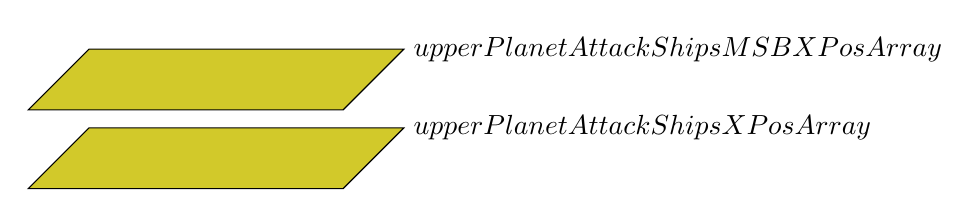
\begin{tikzpicture}
      \draw[fill=yellow!80!black] (0,2,0) -- (4,2,0)--(4,2,2)--(0,2,2)--cycle;
      \node[right] at (4,2,0) {$\icode{upperPlanetAttackShipsXPosArray}$};
      \draw[fill=yellow!80!black] (0,3,0) -- (4,3,0)--(4,3,2)--(0,3,2)--cycle;
      \node[right] at (4,3,0) {$\icode{upperPlanetAttackShipsMSBXPosArray}$};
      \end{tikzpicture}
    \end{adjustbox}

  }
\end{figure}

Then we pop the rest of the items one by one and assign them to the new ship. We ignore the sprite's MXB offset if it is
zero:
\begin{lstlisting}[caption=\icode{PLA} remove the top item from the stack and stores it in \icode{A}.]
        PLA
        BEQ MSBXPosOffsetIzZero

        LDA attackShipsMSBXPosOffsetArray + $01,X
MSBXPosOffsetIzZero   
        STA upperPlanetAttackShipsMSBXPosArray + $01,Y
        PLA
        STA upperPlanetAttackShipsXPosArray + $01,Y
        PLA

        ; Byte 8 of Wave Data gets loaded now. Bytes 8 and 9
        ; contain the hi/lo ptrs to the alternate enemy data.
        LDY #$07
        JMP UpdateWaveDataPointersForCurrentEnemy
\end{lstlisting}

Now that we have set up the positional data for the new enemy we load all its other features from the data pointed
to by Byte 8-9:

\begin{lstlisting}[caption= ]
        ; Byte 8 of Wave Data gets loaded now. Bytes 8 and 9
        ; contain the hi/lo ptrs to the alternate enemy data.
        LDY #$07
        JMP UpdateWaveDataPointersForCurrentEnemy
\end{lstlisting}

Let's take a closer look at this routine \icode{UpdateWaveDataPointersForCurrentEnemy}. What it does in this
instance is take the address pointed to by Bytes 8 and 9 and load the data there using the routine
\icode{GetWaveDataForNewShip}. To be used in this way the values in Bytes 8 and 9 are combined and treated
as an address in memory. For example if Byte 8 contains \icode{\$70} and Byte 9 contains \icode{\$13} they
are treated as providing the address \icode{\$1370}. This is the location where the enemy data for
\icode{planet1Level8Data} is kept so that is what is loaded.



\begin{table}[H]
  {
    \setlength{\tabcolsep}{3.0pt}
    \setlength\cmidrulewidth{\heavyrulewidth} % Make cmidrule = 
    \begin{adjustbox}{width=7cm,center}
      \begin{tabular}{rrll}
        \toprule
        Planet &   Level & Byte 6    & Bytes 7-8                   \\
        \midrule
        1 &      11 & \$03       & smallDotWaveData         \\
        1 &      14 & \$03       & planet1Level8Data        \\
        2 &      19 & \$0C       & landGilbyAsEnemy         \\
        3 &       4 & \$04       & gilbyLookingLeft         \\
        3 &       6 & \$04       & planet3Level6Additional  \\
        4 &      19 & \$01       & planet4Level19Additional \\
        5 &       3 & \$01       & planet5Level3Additional  \\
        5 &       5 & \$05       & planet5Level5Additional  \\
        5 &      14 & \$06       & llamaWaveData            \\
        \addlinespace
        \bottomrule
        \multicolumn{4}{@{}l@{}}{Byte 6 : Whether a specific attack behaviour is used.}\\
        \multicolumn{4}{@{}l@{}}{Bytes 7-8 : Lo and Hi Ptr for alternate enemy mode}\\
      \end{tabular}

    \end{adjustbox}

  }\caption{Actual use of Bytes 6, 7, and 8. Note that the value in Byte 6 doesn't matter, as long as it's non-zero.}
\end{table}


\section{Bytes 22-23: The Bytes of Death}
\begin{figure}[H]
  {
    \setlength{\tabcolsep}{3.0pt}
    \setlength\cmidrulewidth{\heavyrulewidth} % Make cmidrule = 
	\centering
	\def\MULTICOLORONE{white}
	\def\MULTICOLORTWO{red}
	\def\SPRITECOLOR{gray}
	\begin{subfigure}{0.3\textwidth}
		\input{sprites/LICKER_SHIP1}
	\end{subfigure}
	\begin{subfigure}{0.3\textwidth}
		\input{sprites/LICKERSHIP2}
	\end{subfigure}
	\begin{subfigure}{0.3\textwidth}
		\input{sprites/LICKERSHIP3}
	\end{subfigure}
  }\caption[position=top]{These arseholes.}
\end{figure}

An irritating early hurdle in Iridis Alpha's gameplay is the behaviour of the lickerships in the game's third level.
When shot the enemies turn into lickerships that seek out the player and then stick to them, sapping the player's energy
until they lose a life. This behavious is defined by Bytes 22 and 23. 

\begin{lstlisting}
lickerShipWaveData = $1118
  ..
  ; Byte 22 (Index $16): Stickiness factor, does the enemy stick to the player
  ; sapping their energy if they're near them?
  .BYTE $01
  ; Byte 23 (Index $17): Does the enemy gravitate quickly toward the player when its
  ; been shot? (Typical lickership behaviour)
  .BYTE $01
  ..
\end{lstlisting}

Implementing each of these is relatively straighforward. Since the gilby is always in the centre of the screen (on the
X axis at least), all an enemy has to do is figure out whether the gilby is above or below it and move in that direction.
If we leave out the slightly complicated logic to figure out where the gilby is relative to us, we are left with this:

\begin{lstlisting}
MaybeQuicklyGravitatesToGilby
  ; Byte 23:  Does the enemy gravitate quickly towards the gilby when it is shot?
  LDY #$17
  LDA (currentShipWaveDataLoPtr),Y
  BEQ MaybeStickyAttackShipBehaviour
  ...
  ; Figure out the relative position of the gilby and
  ; store it in positionRelativeToGilby
  ...
  ; Now decide whether to move up or down.
  CMP positionRelativeToGilby
  BEQ NoVerticalMovementRequired
  BMI MoveDownToGilby
MoveUpToGilby
  DEC yPosMovementForUpperPlanetAttackShips,X
  DEC yPosMovementForUpperPlanetAttackShips,X
MoveDownToGilby
  INC yPosMovementForUpperPlanetAttackShips,X
NoVerticalMovementRequired
  LDA indexForActiveShipsWaveData,X
  TAX
\end{lstlisting}

Sticking to the gilby involves the same logic but along the horizontal axis. After all if we're sticking to the gilby
we want to stay in the centre of the screen.

\begin{lstlisting}
MaybeStickyAttackShipBehaviour   
  ; Byte 22: Does the enemy have the stickiness behaviour?
  LDY #$16
  LDA (currentShipWaveDataLoPtr),Y
  BEQ MaybeSwitchToAlternateEnemyPattern
  ...
  ; Figure out the relative position of the gilby and
  ; store it in positionRelativeToGilby
  ...
  CMP positionRelativeToGilby
  BMI MoveRightToGilby
MoveLeftToGilby   
  DEC xPosMovementForUpperPlanetAttackShip,X
  DEC xPosMovementForUpperPlanetAttackShip,X
MoveRightToGilby   
  INC xPosMovementForUpperPlanetAttackShip,X
NoHorizontalMovementRequired   
  LDA indexForActiveShipsWaveData,X
  TAX
\end{lstlisting}

\section{Byte 35: Energy Multiplier}
When an enemy is struck this byte contains the multiplier applied to the player's energy boost:

\begin{lstlisting}
IncreaseEnergyTopOnly
    LDY #$23
    LDA (currentShipWaveDataLoPtr),Y
    BEQ NormalTopEnergyIncrease
    STA energyChangeCounter
EnergyTopIncreaseLoop
    JSR IncreaseEnergyTop
    DEC energyChangeCounter
    BNE EnergyTopIncreaseLoop
    RTS

NormalTopEnergyIncrease
    JMP IncreaseEnergyTop
    ;Returns
\end{lstlisting}

The above is for the top planet energy counter, the logic for the bottom planet is identical:

\begin{lstlisting}
IncreaseEnergyBottomOnly
    LDY #$23
    LDA (currentShipWaveDataLoPtr),Y
    BEQ NormalBottomEnergyIncrease
    STA energyChangeCounter
EnergyBottomIncreaseLoop
    JSR IncreaseEnergyBottom
    DEC energyChangeCounter
    BNE EnergyBottomIncreaseLoop
    RTS

NormalBottomEnergyIncrease
    JMP IncreaseEnergyBottom
    ;Returns
\end{lstlisting}

\subfile{titlescreen/energy_tilesheet}

Actually writing the updated energy level to the screen uses the tileset above in the routine
\icode{IncreaseEnergyTop}:
\begin{lstlisting}
IncreaseEnergyTop
    STX temporaryStorageForXRegister
    LDX currEnergyTop
    DEC SCREEN_RAM + LINE22_COL3,X
    LDA SCREEN_RAM + LINE22_COL3,X
    CMP #$7F
    BNE b547B
    ; Note the reference to the index $80 of the first tile in the set above.
    LDA #$80 
    STA SCREEN_RAM + LINE22_COL3,X
    INX
    STX currEnergyTop
    CPX #$08
    BEQ GilbyDiesFromExcessEnergy
    LDA #$87
    STA SCREEN_RAM + LINE22_COL3,X
    BNE b547B
\end{lstlisting}

Byte 35 also determines the multiplier applied to the energy sapped from the player in the 
event of a collision with the enemy:

\begin{lstlisting}
UpdateEnergyLevelsAfterCollision
    ; Check if the enemy saps energy from the gilby?
    LDY #$23
    LDA (currentShipWaveDataLoPtr),Y
    BEQ NoMultiplierAppliedToCollision

    LDA #<shipCollidedWithGilbySound
    STA primarySoundEffectLoPtr
    LDA #>shipCollidedWithGilbySound
    STA primarySoundEffectHiPtr
    JSR ResetRepetitionForPrimarySoundEffect
    LDA #$0E
    STA gilbyExploding
    LDA #$02
    STA starFieldInitialStateArray - $01
    LDA currentGilbySpeed
    EOR #$FF
    CLC
    ADC #$01
    STA currentGilbySpeed

    LDA setToZeroIfOnUpperPlanet
    BEQ EnergyUpdateTopPlanet

    LDA extraAmountToDecreaseEnergyByBottomPlanet
    BNE NoMultiplierAppliedToCollision
    ; Y is still $23.
    LDA (currentShipWaveDataLoPtr),Y
    JSR AugmentAmountToDecreaseEnergyByBountiesEarned
    STA extraAmountToDecreaseEnergyByBottomPlanet
    BNE NoMultiplierAppliedToCollision

EnergyUpdateTopPlanet   
    LDA extraAmountToDecreaseEnergyByTopPlanet
    BNE NoMultiplierAppliedToCollision
    ; Y is still $23.
    LDA (currentShipWaveDataLoPtr),Y
    JSR AugmentAmountToDecreaseEnergyByBountiesEarned
    STA extraAmountToDecreaseEnergyByTopPlanet
NoMultiplierAppliedToCollision
    LDY #$1E
    JMP UpdateWaveDataPointersForCurrentEnemy
    ; Returns

\end{lstlisting}

\section{Byte 34: Score for Hitting the Enemy}
This is used to augment the score received for hitting the enemy.
\begin{lstlisting}
    ; Get the points for hitting enemies in this level
    ; from the wave data.
AddPointsForHittingEnemy   
    ; Byte 34
    LDY #$22
    LDA (currentShipWaveDataLoPtr),Y
    ..
    ADC pointsEarnedTopPlanetByte1
    STA pointsEarnedTopPlanetByte1
\end{lstlisting}


